\chapter{Zeitreisen\label{chapter:thema}}
\lhead{Zeitreisen}
\begin{refsection}
\chapterauthor{Sascha Jecklin und Jonas Gründler}
\section{Einleitung}
Das Thema Zeitreisen fasziniert den Menschen schon seit er sich der Zeit bewusst ist. Früh schon entstanden Träume, den Verlauf der Zeit manipulieren zu können. Erste schriftliche und bildliche Belege dafür gab es bereits in der hinduistischen Mythologie und in der buddhistischen Religion. Auch in der modernen Literatur und in der Filmindustrie sind Zeitreisen ein beliebtes Thema. Klassische Beispiele daf\"ur sind: 
\begin{itemize}
    \item Time Machine, H.G.Wells, 1895 
    \item Das Ende der Ewigkeit, Isaac Asimov, 1955
    \item Back to the Future, 1985-1990
    \item Star Trek
    \item Doctor Who
    \item Interstellar
    \item \ldots
\end{itemize}
\section{Was ist eine Zeitreise}
Eine Zeitreise beschreibt eine Bewegung durch die Zeit, abweichend von der eines Bezugssystems. Man unterscheidet dabei von Reisen in die Vergangenheit oder in die Zukunft. Insbesondere ersteres wirft Fragen auf. Was geschieht z.B. wenn der Lauf der Dinge wie sie bis anhin bekannt waren geändert wird? Wenn der Reisende in der Vergangenheit auf sich selber trifft, oder noch absurder gar sein altes ``Ich`` ermordet? 
Mathematisch gesehen wird eine Reise in die Vergangenheit ebenfalls ein wenig anspruchsvoller. Hier beschränken wir uns daher auf Reisen in die Zukunft. 

Natürlich könnte man später argumentieren, dass sich bei gleichbleibender Theorie die Bezugssysteme vertauschen lassen. So könnte man ein Objekt seiner Wahl reisen lassen und sich selber als Bezugssystem sehen. Dies entspricht aber nicht einer Reise in die Vergangenheit sondern lediglich ``weniger schnellem altern``. Das zeitreisende  Objekt könnte trotz Zeit\"anderung immer nur älter sein als zu Beginn der Betrachtung. Obwohl der Beobachter in seinem Bezugssystem einiges schneller gealtert wäre.

Es stellt sich nun die Frage, wie wir mathematisch gesehen eine Zeitreise definieren. Im Abschnitt XXXXXX führten wir den Begriff der Eigenzeit ein. Sie beschreibt die Zeit, welche im Bezugssystem des Reisenden aus der Sicht eines Beobachters vergeht.

Nun müssen wir noch ausformulieren wie wir die Abweichungen von der Eigenzeit erreichen wollen. Eine Dehnung der Zeit, die sogenannte Zeitdilatation, erreicht man entweder durch Geschwindigkeit oder Gravitation. Geschwindigkeit setzt eine zuvorkommende Beschleunigung voraus. Wir wissen bereits, dass Beschleunigung und Gravitation einhergehen. Daher kommt es nicht all zu \"uberaschend, dass wenn das Eine auch das Andere einen Einfluss haben muss.

Wie wir sehen werden bringen schon kleinste \"Anderungen eine Zeitänderung mit sich. Da die praktische Anwendung in diesem Kapitel im Vordergrund steht, interessieren uns in erster Linie natürlich signifikante Unterschiede. Erst doppelt oder sogar zehnmal-schneller vergehenden Zeiten w\"urden uns Effekte best\"atigen, welche man uns in Science Fiction Filmen und Romanen verspricht.

\subsection{Geschwindigkeit}
Eine M\"oglichkeit eine Zeitdillatation zu bewirken ist durch hohe Geschwindigkeit. Wenn sich eine Person relativ zu einem Bezugssystem schnell bewegt, vergeht f\"ur diese Person die Zeit im Vergleich zum Bezugssystem langsamer. Die Ver\"anderung wird durch den Lorentzfaktor beschrieben, welcher sich aus der Lorentztransformation herleiten l\"asst. Er beschreibt das Verh\"altnis zwischen der Eigenzeit und der Zeit des Bezugssystems.
\begin{equation}
    \gamma=\frac{1}{\sqrt{1-\displaystyle\frac{v^2}{c^2}}} 
\end{equation}
Die Eigenzeit ist also:
\begin{equation}
    \tau
    =
    \int_{}^{}\frac{1}{\gamma}dt=\int_{}^{}\sqrt{1-\frac{v^2}{c^2}}dt
    =
    \frac{1}{c}\int_{}^{}\sqrt{g_{\mu\nu}\dot{x}^{\mu}(s)\dot{x}^{\nu}(s)}ds
\end{equation}
Diese Formel ist in dieser Form noch nicht sehr anschaulich. Sie beschreibt nur, dass eine Metrik mit den jeweiligen Basisvektoren "multipliziert" werden muss(Einsteinsche Summenkonvention). Von dem Ganzen die Wurzel ziehen und dann noch integrieren.
Durch das verwenden der Minkowski-Metrik, welche Raum und Zeit miteinander verbindet, und der Basisvektoren $t, x, y, z$ l\"asst sich eine verst\"andliche Form herleiten. 
Minowski-Metrik:
\begin{equation}
    g_{\mu\nu}=
    \begin{pmatrix}
        -1 & 0 & 0 & 0 \\
        0 & 1 & 0 & 0 \\
        0 & 0 & 1 & 0 \\
        0 & 0 & 0 & 1
    \end{pmatrix}
\end{equation}
Standard Vierervektor:
\begin{align*}
    x^{0}=c \cdot t,
    x^{1}=x,
    x^{2}=y,
    x^{3}=z,
\end{align*}
Ein wenig Umstellen und vereinfachen und man kommt auf diese Form:
\begin{equation}
    \tau
    =
    \frac{1}{c}\int_{}^{}\sqrt{-(-c^2\dot{t}(s)^{2}+\dot{x}(s)^{2}+\dot{y}(s)^{2}+\dot{z}(s)^{2})}ds
\end{equation}
Je nachdem wie die Bewegung gew\"ahlt wird, fallen einer oder mehrere der Koordinaten $x, y, z$ weg.
Hier ein Beispiel bei welchem nur eine Geschwindigkeit in x-Richtung vorhanden ist ($c=$Lichtgeschwindigkeit, u beschreibt den Bruchteil):
\begin{align*}
     t(s)=1\cdot s, \dot{t}(s)=1,
 	 x(s)=u\cdot c \cdot s, \dot{x}(s)=u\cdot c,
     y(s)=0, \dot{y}(s)=0,
     z(s)=0, \dot{z}(s)=0
\end{align*}
\begin{align*}
    \tau
    &=
    \frac{1}{c}\int_{}^{}\sqrt{-(-c^2\dot{t}(s)^2+\dot{x}(s)^2)}ds 
    =
    \frac{1}{c}\int_{}^{}\sqrt{-(-c^2 +(u\cdot c)^{2}}ds\\
    &=
    \frac{s\sqrt{c^2+(u\cdot c)^{2}}}{c} 
    =
    s\sqrt{1-\frac{u^2\cdot c^2}{c^2}}
\end{align*}
Welches die einfachste Form einer Zeitdilatation darstellt.
Hier ein Zahlenbeispiel bei welchem willkürliche Werte gew\"ahlt wurden:
$s=5000, u=0.2$ 
\begin{align*}
    t(s)=s, \dot{t}(s)=1,
    x(s)=0.2c \cdot s, \dot{x}(s)=0.2c,
    y(s)=0, \dot{y}(s)=0,
    z(s)=0, \dot{z}(s)=0,
\end{align*}
Diese Werte in die Gleichung eingesetzt ergeben
\begin{align*}
    \tau
    &=
    \frac{1}{c}\int_{s_{a}}^{s_{b}}\sqrt{-(-c^2\dot{t}(s)^2+\dot{x}(s)^2)}ds
    &=
    \frac{1}{c}\int_{0}^{5000}\sqrt{-(-c^2+((0.2c)^2))}ds\\
    &=
    5000\sqrt{1-\frac{u^2 c^2}{c^2}} = 4898.98
\end{align*}
Dieses Beispiel zeigt auch, dass eine relevante Zeitverlangsamung erst bei sehr hohen Geschwindigkeiten erreicht wird.
\begin{figure}[H]
    \centering
    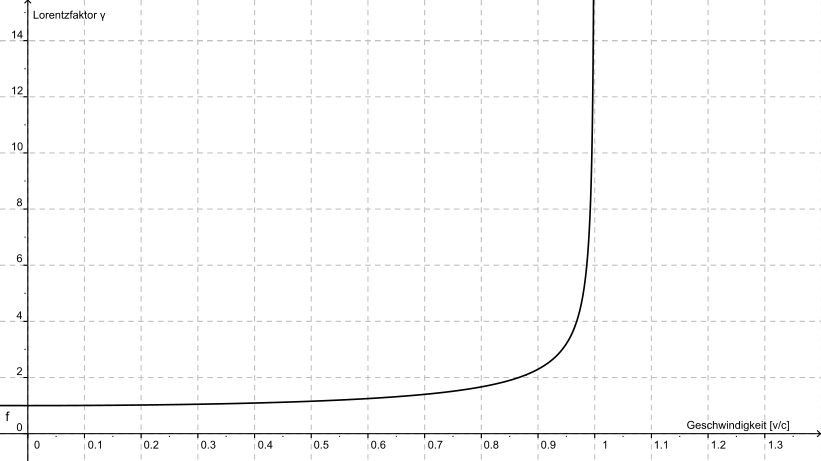
\includegraphics[width=\hsize]{zeitreisen/Lorentzfaktor.jpg}
    \caption{Ver\"anderung des Lorentzfaktor in Abh\"angigkeit der Geschwindigkeit%
        \label{skript:geodaten:fig:transport}}
\end{figure}
\subsection{Gravitation}

	In diesem Kapitel beschäftigen wir uns mit dem Einfluss der Gravitation auf die Zeit. Gravitation muss durch eine Krümmung des Raumes beschrieben werden. Erkennen lässt sich die Gravitation z.B. an der Anziehungskraft der Erde. Alles wird mit $g=9.81\frac{m}{s^2}$ in Richtung Erdmittelpunkt beschleunigt. $F=\frac{KMm}{r^2}$
	Die Beschleunigung ist also unabhängig von der Masse.
	Ein beschleunigtes Koordinatensystem kann zwar durch eine Koordinatentransformation erreicht werden, doch diese ist keine Lorentztransformation und lässt sich nicht durch die Minkowski-Metrik darstellen.
	
	Der Ansatz $ -c^2dt^2 + dx^2 + dy^2 + dz^2$ genügt nicht mehr. Wir müssen also Metriken und Transformationen zulassen, welche von der Minkowski-Metrik und der Standarttransformation abweichen.
	
	Eine Metrik, welche wir für unsere Zwecke benützen können, ist die Schwarzschild-Metrik. Sie berücksichtigt die Gravitation, durch eine Krümmung des Raumes dargestellt, und beschreibt so Gravitationsfelder in der nähe von massereichen Objekten. Diese Lösung wurde von Karl Schwarzschild nur wenige Monate nach der Präsentierung der Einsteinschen Feldgleichungen gefunden. Aus ihr lassen sich Bewegungsgleichungen von Körpern in einem Gravitationstrichter herleiten.
	
	Die Schwarzschildmetrik in Vektordarstellung:

    \begin{equation}
		g_{\mu\nu}=
		\begin{pmatrix}
		-\biggl(-1-\frac{r_{g}}{r}\biggr) & 0 & 0 & 0 \\
		0 & \frac{1}{\displaystyle1-\frac{r_{g}}{r}} & 0 & 0 \\
		0 & 0 & r^{2} & 0 \\
		0 & 0 & 0 & r^{2}\sin^{2}(\vartheta)
		\end{pmatrix}
	\end{equation}
Der Vierervektor in Kugelkoordinaten:
	\begin{align*}
		x^{0}=c\cdot t
		x^{1}=r
		x^{2}=\vartheta
		x^{3}=\varphi
	\end{align*}
	Daraus lässt sich die Längenmessung zusammenstellen. Die Schwarzschild-Metrik wird im Kapitel (:::LABEL:::) hergeleitet
	\begin{equation}
	ds^2
	=
	-\biggl(1-\frac{r_g}r\biggr)c^2dt^2
	+
	\frac{1}{\displaystyle 1-\frac{r_g}r}\,dr^2 
	+
	r^2d\vartheta^2 
	+ 
	r^2\sin^2(\vartheta)d\varphi
	\end{equation}
	$r_g$ beschreibt den Gravitationsradius(Ereignishorizont) des betrachteten Körpers.
	\subsubsection{Bedeutung von $R_{g}$ und Ereignishorizonte}
	Der Ereignishorizont beschreibt in der allgemeinen Relativitätstheorie eine Grenzfläche dar. Er beschreibt die Entfernung ab welcher das Licht nicht mehr aus der Gravitationstrichter entkommen kann. Teilchen die den Ereignishorizont passiert haben, können diesen nicht mehr verlassen. Alles ausserhalb dieses Radius hätte die Möglichkeit zu entkommen, die frage ist nur wie viel Energie benötigt wird. Da Licht nicht mehr entkommen kann nennt man diese Körper auch schwarze Löcher.
	Der Gravitationsradius lässt sich mit \ref{Gravitationsradius} berechnen.
	\begin{equation} \label{Gravitationsradius}
		r_{g}= \frac{2MG}{c^2}
	\end{equation}
    Der Gravitationsradius der Erde beträgt etwa 8.8mm. Wenn wir die Erde also unter  diese 8.8mm komprimieren, würde sie sich in ein schwarzes Loch verwandeln. Ihre Dichte wäre dann so gross, dass nichts mehr der Anziehung widerstehen kann.
	%do vlt no chli was... weiss aber nonig genau was
	
	\section{Realisierbarkeit}
	
	Wie erreichen wir nun eine grössere Zeitdilatation um in der Zeit zu reisen? Entweder mit grosser Geschwindigkeit oder mittels eines Massereichen Objektes. Zeitdilatation durch hohe Geschwindigkeiten zu erreichen ist sehr schwierig, da die benötigte Energie im Quadrat mit der Geschwindigkeit anwächst. Und wie (Figure 1) zeigt, muss für eine grosse Zeitverlangsamung annähernd Lichtgeschwindigkeit erreicht werden. Erst ab ca. $0.9c$ beginnt der Lorentzfaktor wirklich zu wachsen.
	Das bedeutet, dass wir uns auf den Effekt der Gravitation  konzentrieren müssen.
	Doch wir lösen wir dieses Problem? Wir suchen also ein Massereiches Objekt in unserer Umgebung. Die Sonne genügt für unsere Zwecke leider nicht, ihr Schwarzschildradius ist erstens viel zu klein, und zweitens innerhalb des Körpers. Wir suchen also weiter... Schliesslich finden wir Sagittarrius A*, ein supermassives schwarzes Loch im Zentrum unserer Milchstrasse. Dieses sollte für unsere Zwecke genügen. 
	Doch hier beginnen die Probleme. 
	Sagittarrius A* ist 26'000 Lichtjahre von uns entfernt, das bedeutet mit Lichtgeschwindigkeit bräuchten Wir 26'000 Jahre bis wir am Ziel ankommen. Die Hoffnung wäre nun, dass sich durch eine hohe Fluggeschwindigkeit und die daraus resultierende Zeitdehnung, die benötigte Zeit signifikant reduziert. 
	Nehmen wir nun an wir fliegen mit 0.5-facher Lichtgeschwindigkeit ins Zentrum unserer Milchstrasse. Die Eigenflugzeit im Raumschiff wäre immer noch
	\begin{align*}
	\tau
	&= 
	\int_{}^{26000}\frac{1}{\gamma}dt=\int_{}^{26000}\sqrt{1-\frac{v^2}{c^2}}dt
	= 
	\frac{1}{c}\int_{0}^{26000}\sqrt{-(-c^2+(0.5c)^2)}ds\\
	&=
	\biggl[s\sqrt{1-\frac{(0.5c)^{2}}{c^2}}\biggr]_0^{26000}
	=
	22516.7.
	\end{align*}
	was also grosszügig gerundet immer noch 22500 Jahre dauern würde. 
	Wir müssen Mit unserem Projekt also warten, bis Geschwindigkeiten von 0.99c mit Raumschiffen Erreicht werden können. Doch auch mit 0.99c würde die Reise noch 3600 Jahre Dauern. Die Energie die benötigt würde, um ein Raumschiff auf diese Geschwindigkeit zu beschleunigen, vernachlässigen wir hier. Das ist ein anderes Problem welches noch gelöst werden muss.
	Wir verschieben unser Projekt also in hypothetische und stellen uns vor wir wären bereits da.
	
	\section{Am Ziel\dots Was nun?}
	
	Wenn wir nun also diese Reise auf uns genommen haben, und Sagittarrius A* wirklich erreichen, öffnen sich uns zwei Möglichkeiten:
	\begin{itemize}
		\item eine gesteuerte Bahn
		\item wir lassen uns "fallen"
	\end{itemize}
	Eine gesteuerte Kreisbahn um das schwarze Loch bringt die besten Resultate, da wir eine Kreisbahn sehr nahe am Ereignishorizont wählen können. Das Ganze wäre jedoch sehr Energieaufwändig, da wir mit Steuerdüsen unseren Absturz in den Ereignishorizont verhindern müssen. Je nach Geschwindigkeit und Abstand zum schwarzen Loch wird mehr oder weniger Energie benötigt.
	
	Die zweite Möglichkeit wäre, dass wir uns, wenn wir angekommen sind "fallenlassen" und sehen was passiert. So können wir je nach Anfangsgeschwindigkeit, Abstand und £Position verschiedene Bahnen erreicht werden. Vom Absturz in den Ereignishorizont bis zu einer Bahn auf der wir der Gravitation des schwarzen Lochs entkommen und uns in die weiten des Weltalls verabschieden. Beides sind eher unangenehme Szenarien. 
	Wie finden wir also eine Bahn möglichst nahe an der Singularität, ohne das eines dieser zwei Ereignisse auftritt?
	Lösung unseres Problem sind die Geodätengleichungen, welche uns aufgrund der Anfangsbedingungen eine Bahn berechnen lassen.
	
	
	\section{Geodätenbahnen}
	
	Mit den Geodäten lassen sich nun physikalisch korrekte Bahnen um ein schwarzes Loch herleiten. Dafür benötigen wir die in Kapitel 3.4 vorgestellte Geodätengleichung	
	\begin{equation}
	\ddot{x}^{\alpha} + \Gamma^{\alpha}_{\mu\nu}\dot{x}^{\mu}\dot{x}^{\nu} = 0
	\end{equation}	
	Wir können nun in der nähe des schwarzen Lochs alle Antriebe ausschalten und uns treiben lassen. Die aktuelle Geschwindigkeit, Position, Richtung und Abstand stellen nun die Anfangsbedingungen dar. Mit einer numerischen Lösung dieser Gleichungen können wir nun Schritt für Schritt die neuen Faktoren ausrechnen. Dazu kommt noch dass wir die Vergehend Zeit auch messen können.
	Wir k\"onnen nun die Gleichung wie folgt umstellen:	
	\begin{equation}
	\ddot{x}^{\alpha} = -\Gamma^{\alpha}_{\mu\nu}\dot{x}^{\mu}\dot{x}^{\nu}
	\end{equation}
	Daraus lässt sich interpretieren, dass die Beschleunigungen, welche für die nächste Position wichtig sind, ein Produkt sind aus den Christoffelsymbolen 2.Art und den zugehörigen Ableitungen.
	Nun können Wir diese Gleichung in die vier Komponenten aufspalten
	\begin{align*}
		\ddot{t}(s) = -\Gamma^{1}_{\mu\nu}\dot{x}^{\mu}\dot{x}^{\nu}\\
		\ddot{r}(s) = -\Gamma^{2}_{\mu\nu}\dot{x}^{\mu}\dot{x}^{\nu}\\
		\ddot{\vartheta}(s) = -\Gamma^{3}_{\mu\nu}\dot{x}^{\mu}\dot{x}^{\nu}\\
		\ddot{\varphi}(s) = -\Gamma^{4}_{\mu\nu}\dot{x}^{\mu}\dot{x}^{\nu}		
	\end{align*}
	Da wir uns in einer Ebene bewegen ist der Winkel$\vartheta = const$ und somit auch seine Ableitungen. Dadurch fällt der   ganze $\ddot{\vartheta}$ Term weg. Das Problem reduziert sich also auf drei Dimensionen.	
	
	%Work in Progress;)
	
	
	\section{Simulation}
	
	%Erklärung sourcecode
	
	\section{fazit}
	
	%üseri erkenntnis us de arbet
	
	


	\printbibliography[heading=subbibliography]
	\end{refsection}

